\chapter{Derivation of Parasite Clearance Times}
\section{Estimating the primary endpoint}
The endpoint of primary importance is PC90, the time to achieve a reduction of the parasitaemia by 90\% of baseline level. The baseline level is the pre-dose parasite count. We have data for parasite counts taken at specific times and therefore will have a measurement of the parasite count at a time when the count was above 90\% of the baseline, followed by one where it where it is below 90\% and hence we need to find an appropriate interpolation to determine a time at which the parasite count was 90\%.

As a first attempt at deriving estimates of PC90 from the data, simple linear polynomial fits to the logarithm of the parasite count with time from first dose are investigated. This is followed by non-linear logistic regression as has been used by others\cite{wootton}. We also look at simple linear or or log-linear interpolation which has also been used for data of this kind\cite{carmello}.
\subsection{Using a transformation of the count}
In the previous chapter it was noted that a logarithmic transformation was appropriate to remove the skew of the parasite count distribution. Figure \ref{raw901M} shows the untransformed parasite count for centre 1 males with a horizontal line indicating the PC90 level and Figure \ref{log901M} shows the log-transformed parasite count.

We can see that the logarithmic transformation reduces the significance of large fluctuations in the parasite count soon after first dose and brings the region around the PC90 level into greater prominence. Consequently, interpolated estimates of PC90 in these log-linear co-ordinates will be more accurate and any regression will be more influenced by data close to the region of interest.  
\begin{figure}[p]
\begin{center}
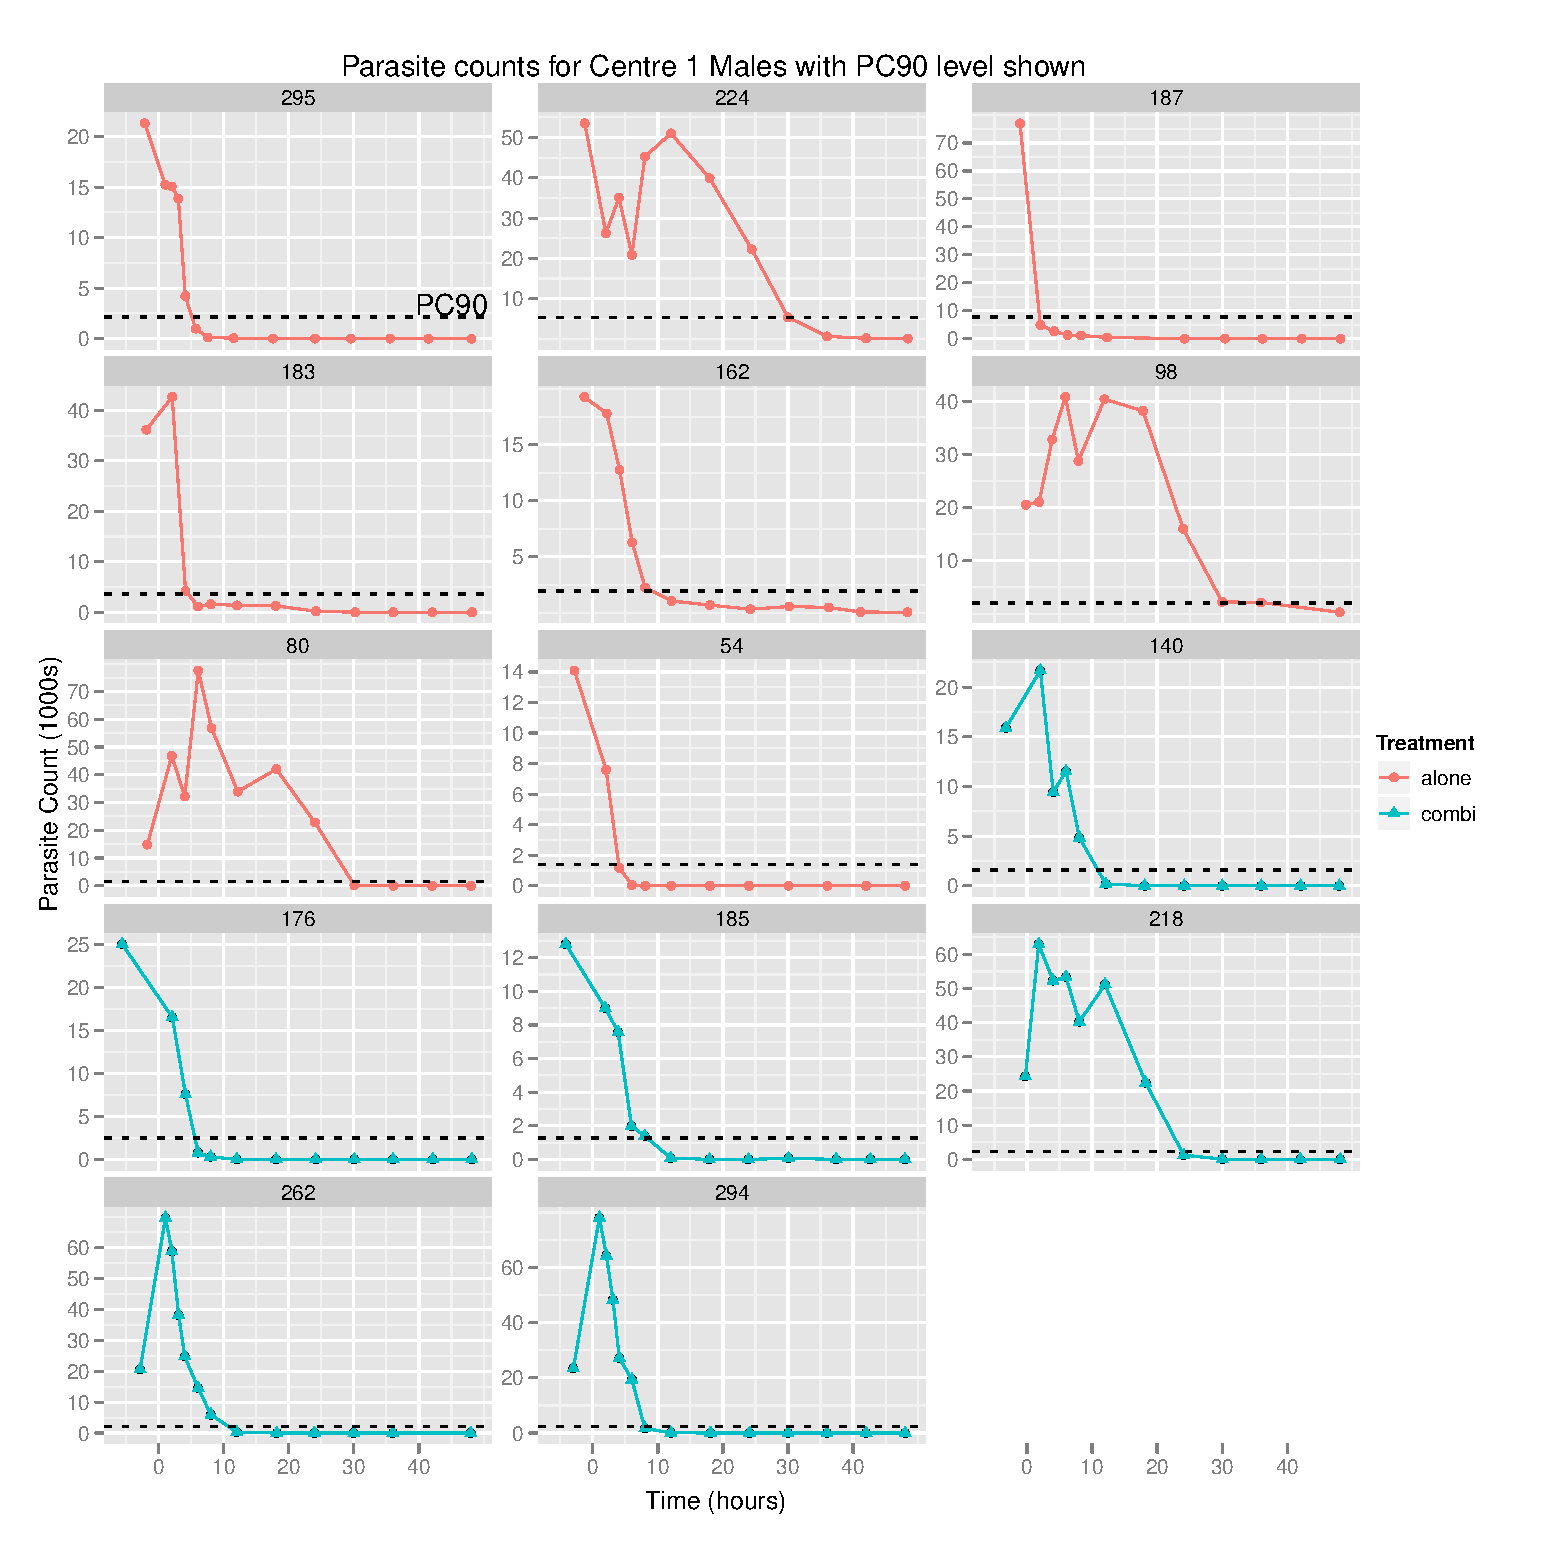
\includegraphics[width=6.1in]{raw901M.eps}
\caption{Untransformed parasite counts with PC90 level shown}
\label{raw901M}
\end{center}
\end{figure}
\begin{figure}[p]
\begin{center}
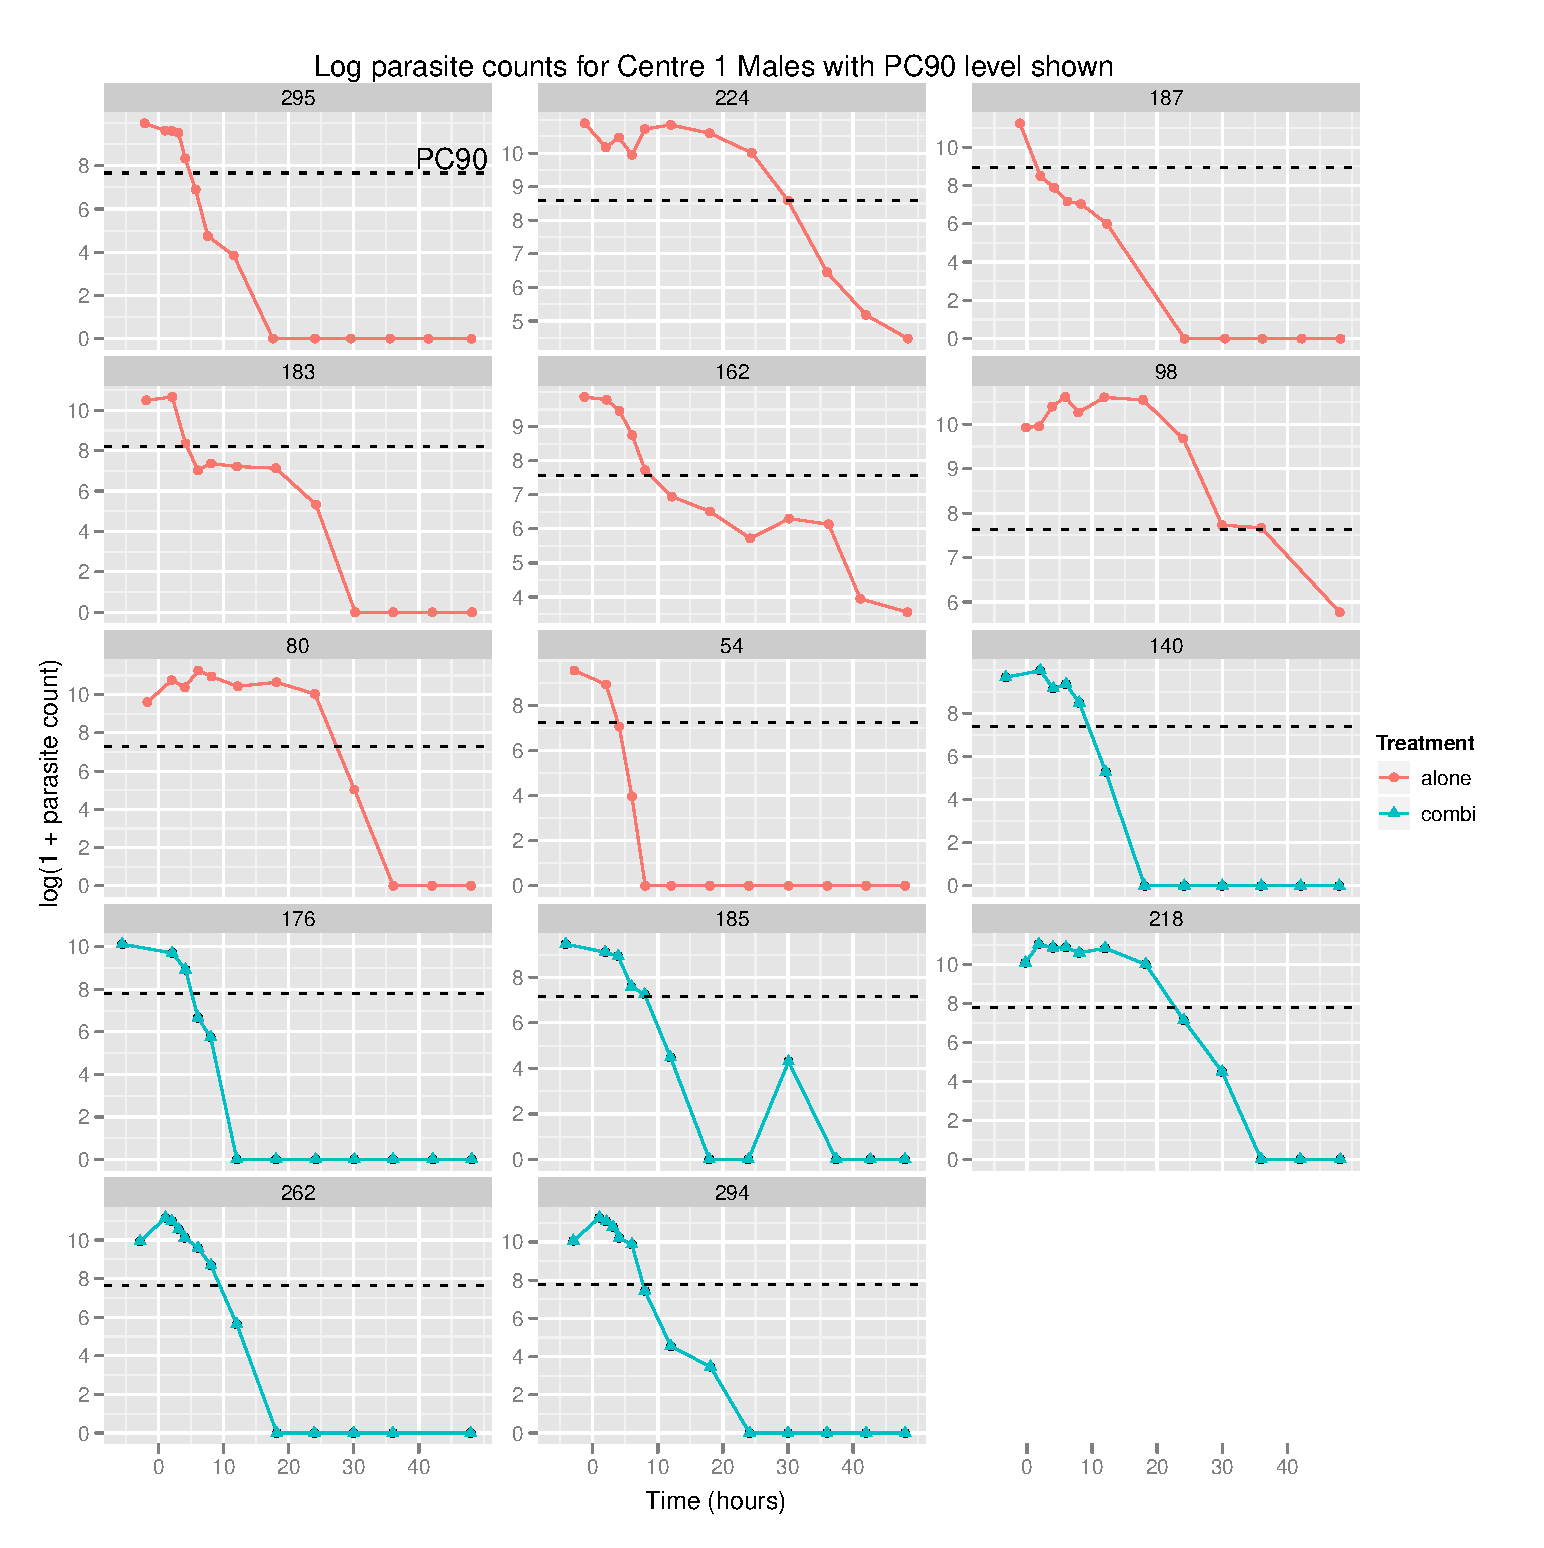
\includegraphics[width=6.1in]{log901M.eps}
\caption{Log parasite counts with PC90 level shown}
\label{log901M}
\end{center}
\end{figure}
\section{Estimation techniques}
\subsection{Polynomial linear regression}
It was found that a cubic was the most suitable model, if we include the data only up to the first 0 parasite count. For some patients where the parasite count drops quickly to 0 a fit that includes the subsequent run of 0s would pull the cubic fit away from the most sensible estimate of PC90. It is more suitable for the purpose of estimating PC90 to only model the drop in the count to 0.

A cubic model was fitted to the log-transformed parasite count $P_{t}$ with time from first dose $t$ as the explanatory variable
$$\log(1+P_{t})=\beta_0+\beta_1t+\beta_2t^2+\beta_3t^3+\epsilon\quad\quad\epsilon\sim N(0,\sigma^2)$$

Figure \ref{cubics} shows the cubic fits to the log parasite count for centre 1, male subjects. It can be seen that the model describes the data fairly well, but it looks as if the combined treatment data is more closely modelled with the single treatment data showing more dispersion about the fitted model. 

Figure \ref{cubicsresid} shows the standardized residuals ($e/\hat{\sigma}$) for the cubic fits. It can be seen that they are normally distributed and show no obvious correlation with time from first dose or with fitted count. The cluster of small magnitude residuals at 0 fitted value occurs because this datum in the fit for each subject is not random but is always 0. Strictly this invalidates the assumptions of the fitted model but there isn't a more suitable choice for determining the shape. The cubic model is really only used as a convenient method of interpolation and we are not interested in the accuracy of the fitted parameters as long as there is no systematic bias. 
\subsubsection*{Determining PC90 from the fitted model}
The value of PC90 i.e. the time t at which the parasite count has fallen to 10\% was found by least-squares i.e. using the \texttt{optimize} function in R to minimise:
$$[log(1+0.1P_0)-\beta_0-\beta_1t-\beta_2t^2-\beta_3t^3]^2$$
where $P_0$ is the pre-treatment parasite count, $t$ is the time from first dose and $\beta_i$ are the fitted coefficients for the models for each of the 43 patients. Table \ref{pc90} shows the values of PC90 derived from the cubic fit to the parasite count by centre, sex and treatment.
\begin{figure}[h]
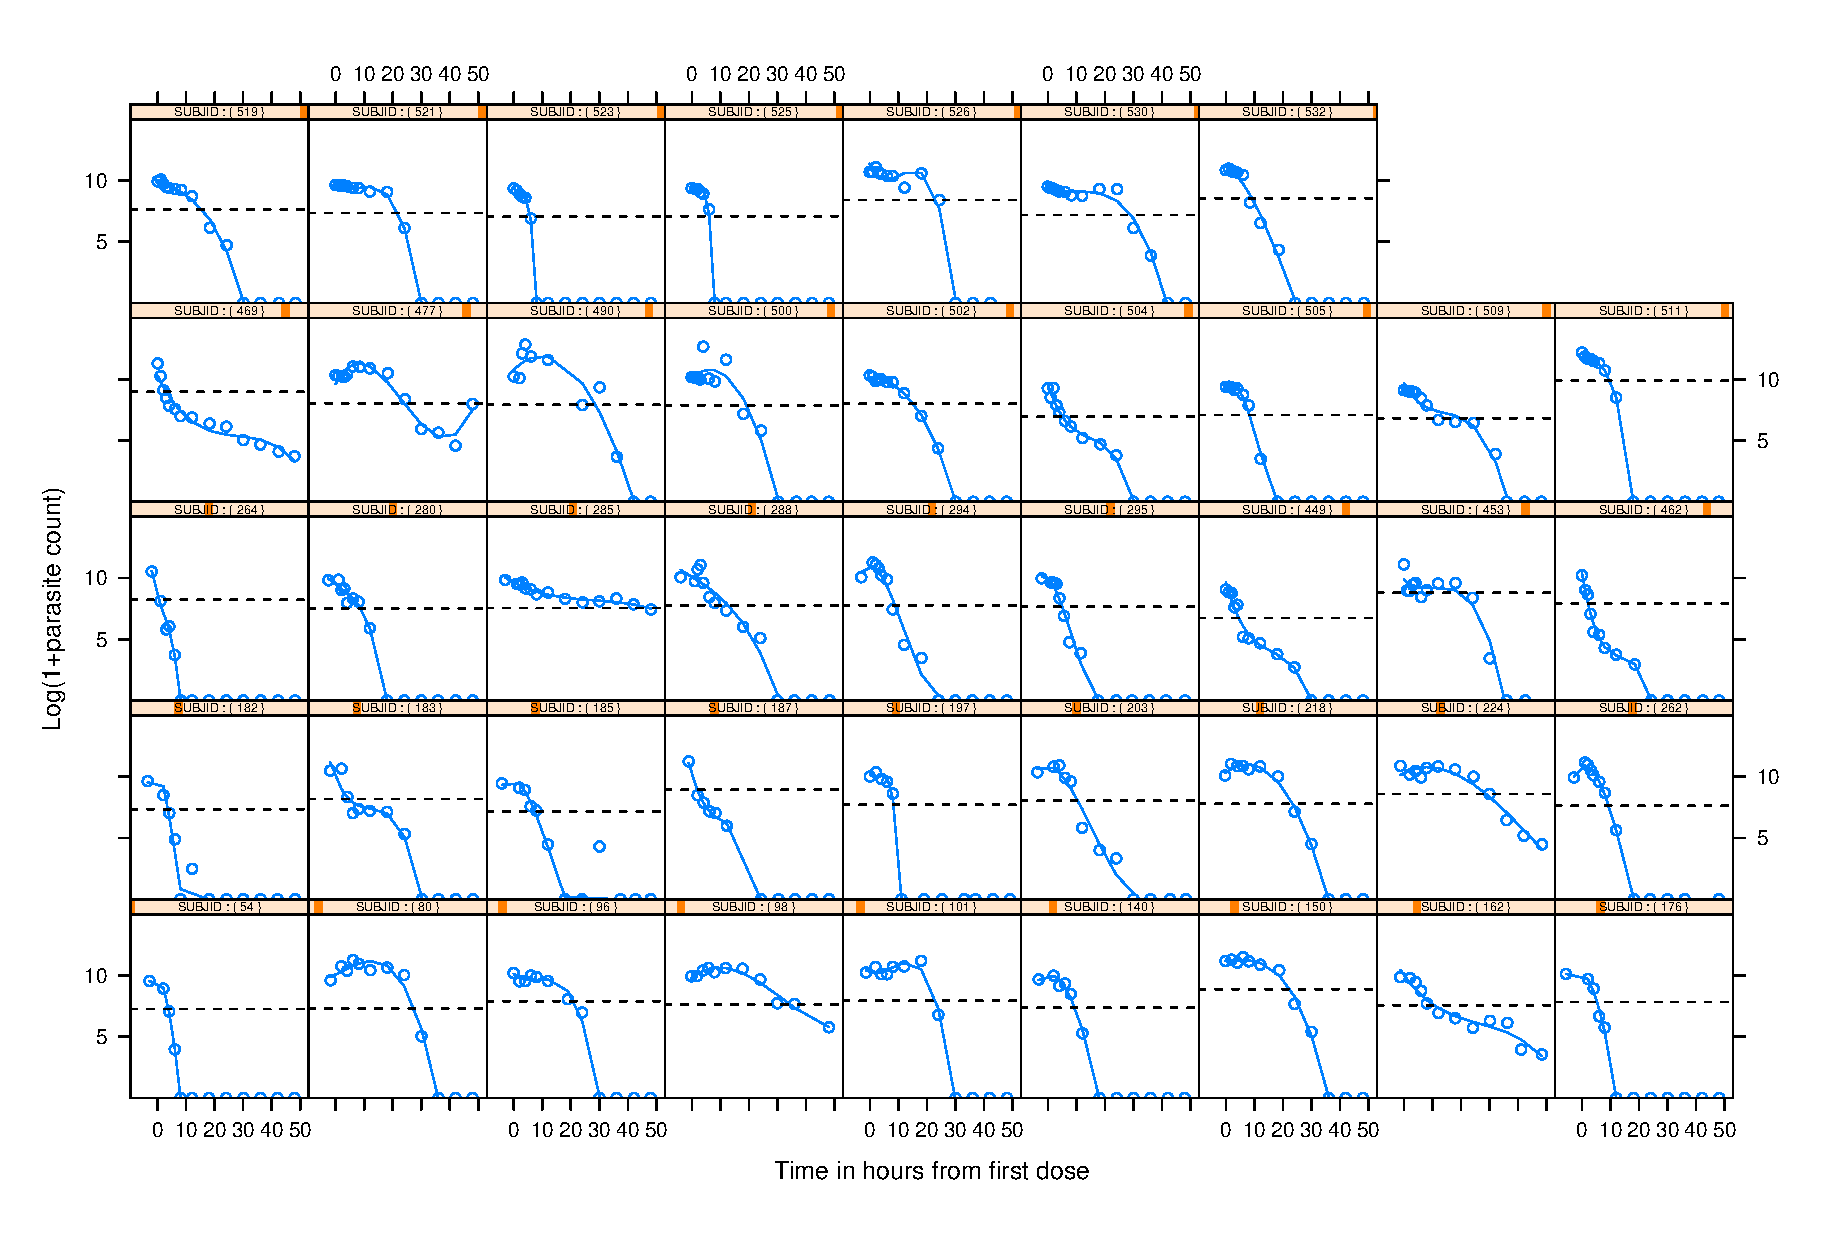
\includegraphics[width=6.1in]{cubics.eps} 
\caption{Cubic fits to log parasite count up to first zero reading}\label{cubics}
\end{figure}
\begin{figure}[h]
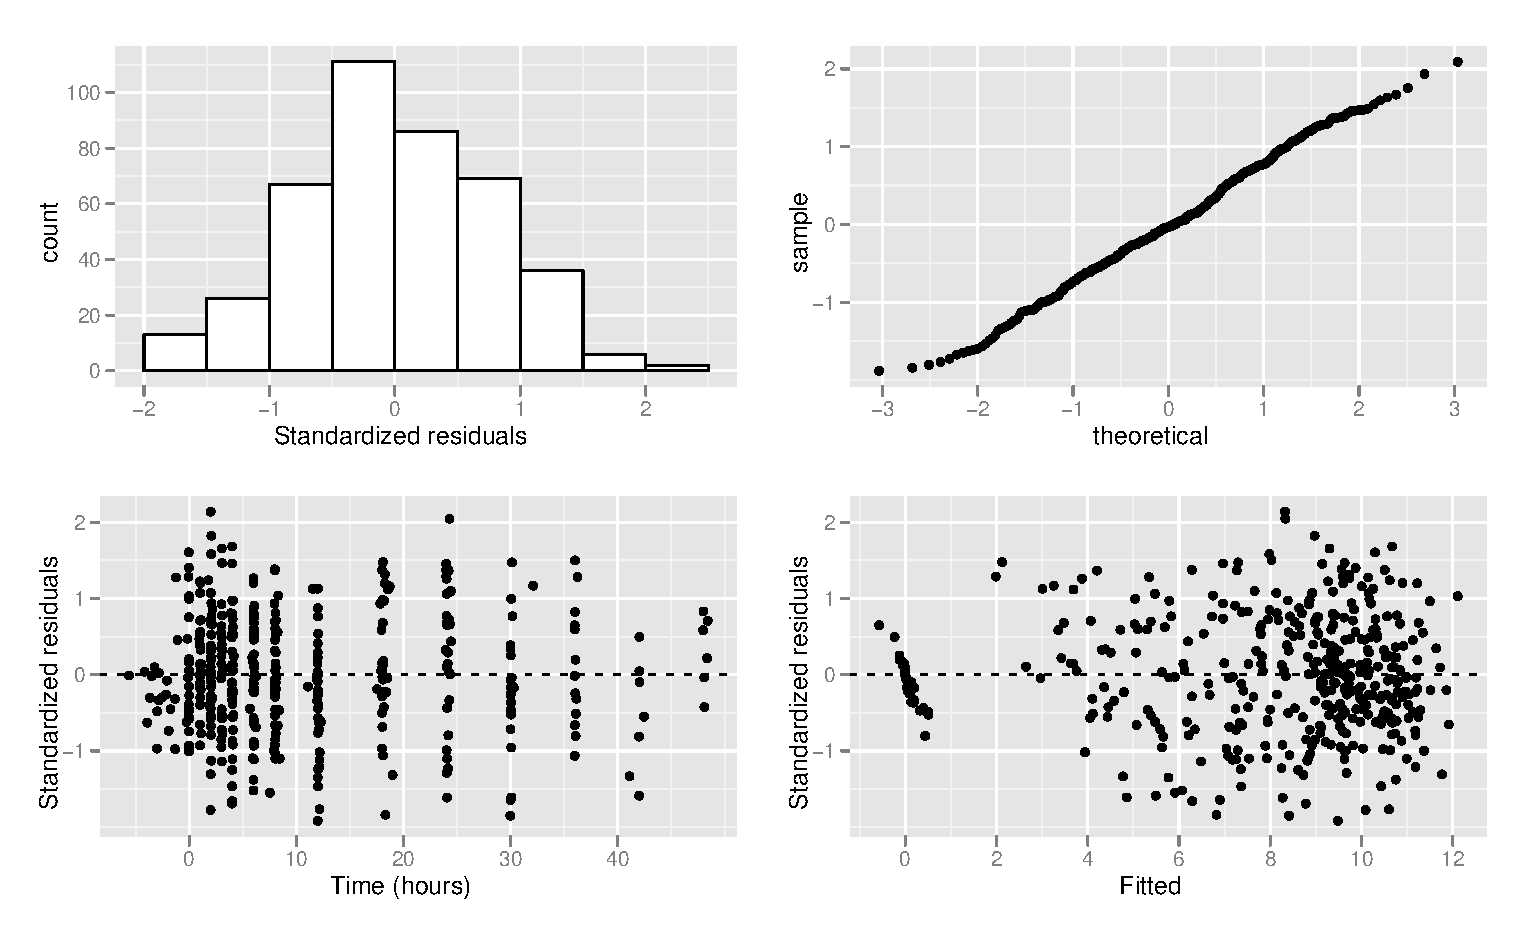
\includegraphics[width=6.1in]{cubicsresid.eps} 
\caption{Standardized residuals for cubic fits}\label{cubicsresid}
\end{figure}
\clearpage
\subsection{Non-linear logistic regression}
The logistic model fitted is
$$\log(1+P_t)=\alpha+\frac{\lambda}{1+e^{-\beta(t-\mu)}}+\epsilon$$
This was fitted to all the data as it can model a drop from an initial count level to a level of 0, unlike the cubic model. $\alpha$ is the lower asymptote which we would expect to be 0. $\alpha+\lambda$ is the upper asymptote which we would generally expect to be $P_0$ except in the cases where there is a marked increase in the parasite count after the first dose. $\beta$ determines the rate of reduction with time and $\mu$ is the point of inflection (maximum rate of reduction). This model was fitted using non-linear least-squares routines in \emph{R} and \emph{SAS}. Logistic fits to the same subjects as the cubic fits in Figure \ref{cubics} are shown in Figure \ref{logistics}.
\subsubsection*{Choosing starting values for the parameters}
Figure \ref{logparms} shows the roles the parameters of the logistic model play in shaping the fitted curve. The non-linear, least-squares fitting routines (the \texttt{nls} function) in \emph{R} can take starting values for the parameters to be estimated.
\begin{figure}[h]
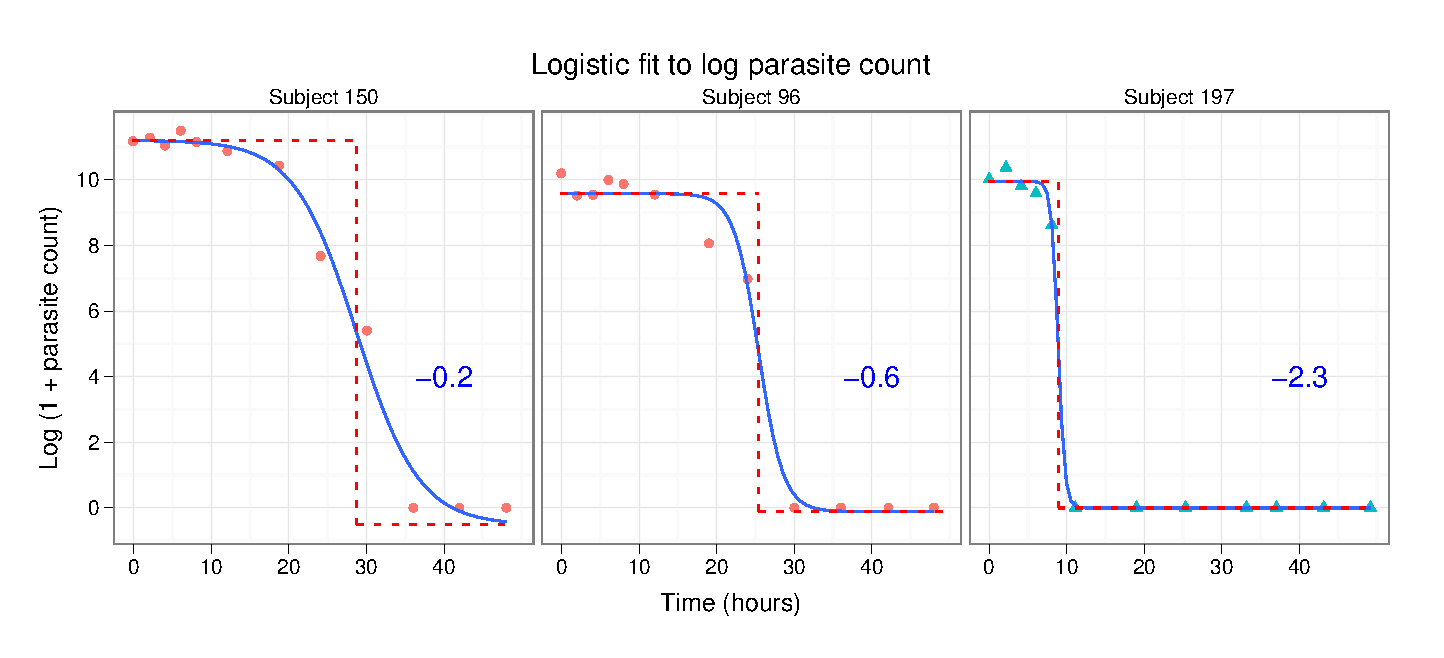
\includegraphics[width=6.1in]{logparms.eps} 
\caption{Illustration of parameters for logistic fits.\newline
The horizontal red lines show $\log(1+P_t)=\alpha$ (lower) and $\log(1+P_t)=\alpha+\lambda$ (upper), the vertical red line shows $t=\mu$ and the coefficient $\beta$ (rate of reduction) is given in blue.}\label{logparms}
\end{figure}

Looking at Figure \ref{logparms} it clearly follows that sensible starting values are:
\begin{itemize}
\item $\alpha$ = the minimum parasite count; usually 0.
\item $\lambda$ = the maximum minus the minimum count; usually the maximum.
\item $\mu$ = the time corresponding to the parasite count closest to halfway between the maximum and minimum counts.
\end{itemize} 
It was found by experimentation that the most suitable starting value for $\beta$ was -0.5, but that the fitting was insensitive to choice of $\beta$ if varied over the range of fitted $\beta$ values observed (and somewhat beyond).
\begin{figure}[p]
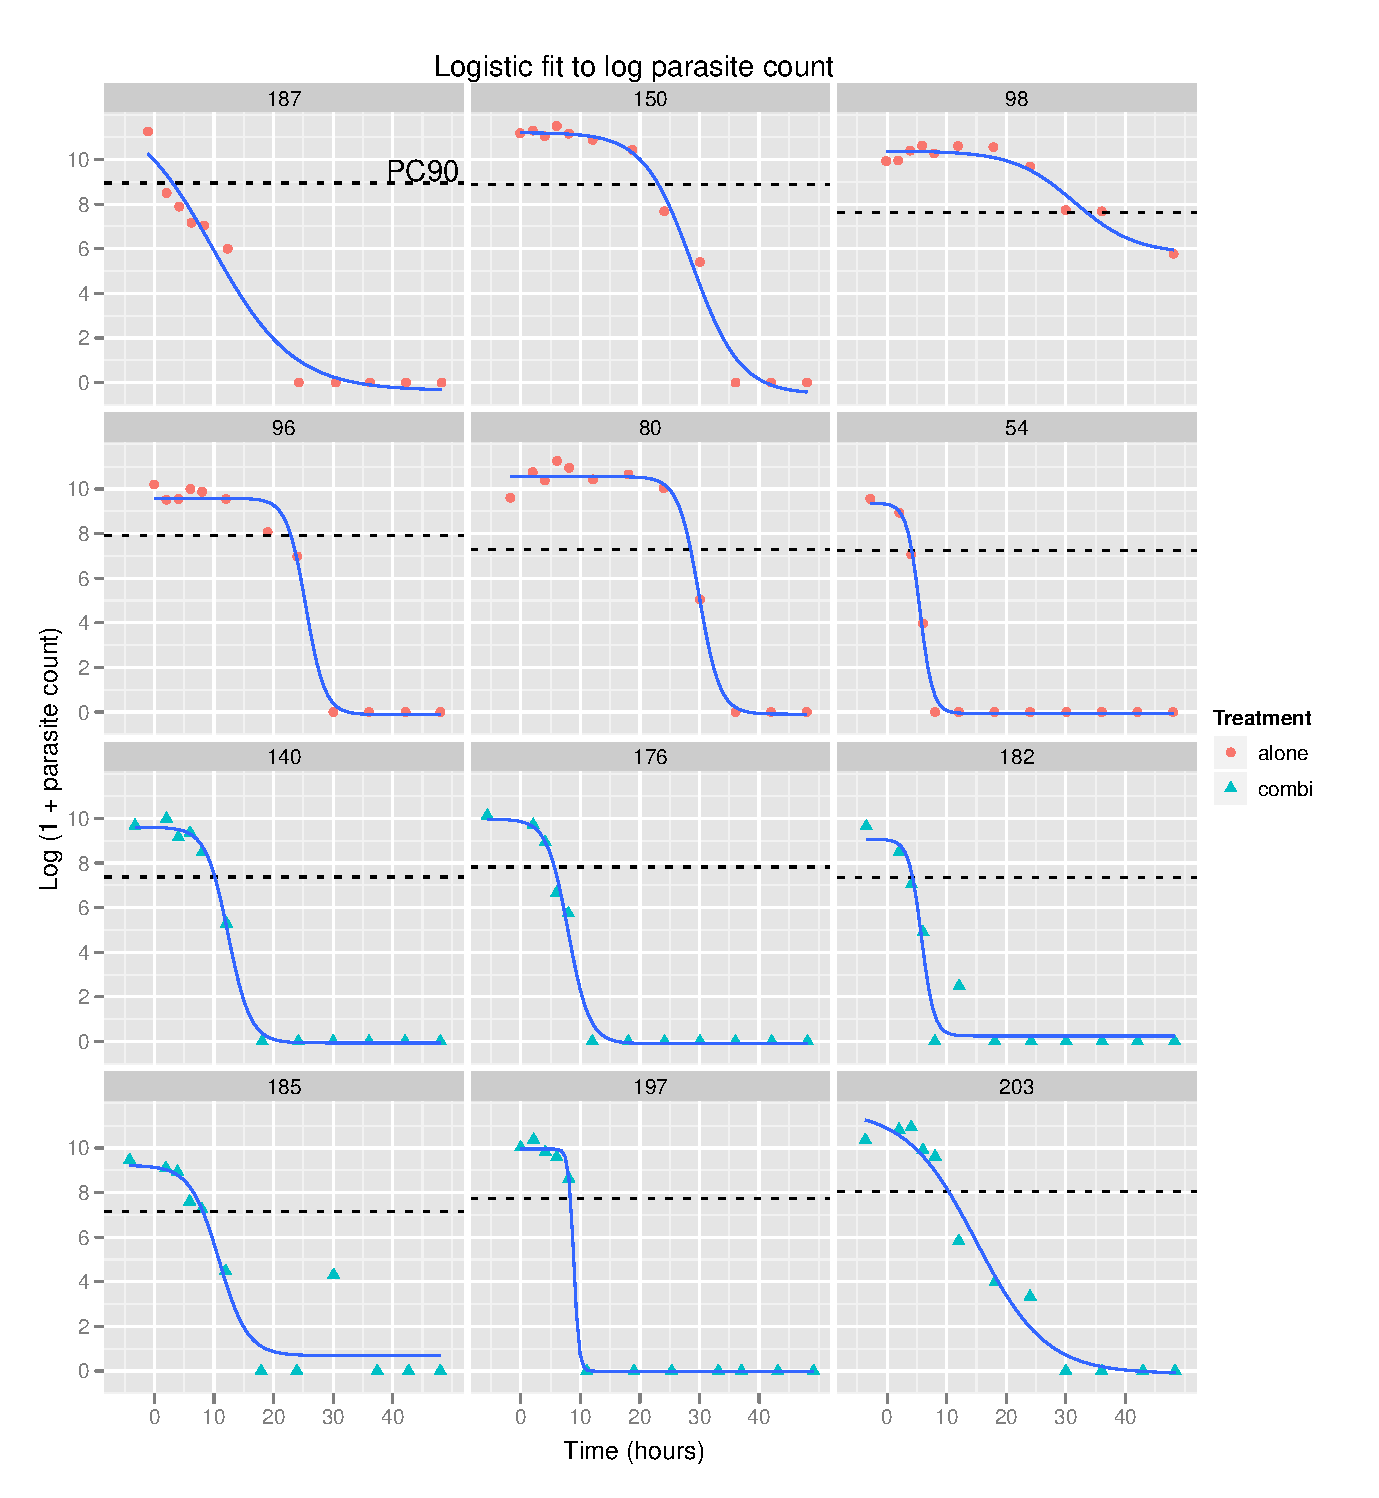
\includegraphics[width=6.1in]{logistics.eps} 
\caption{Logistic fits to log parasite count}\label{logistics}
\end{figure}
\subsubsection*{Failure of logistic fitting}
Despite careful selection of starting parameters, it was found for several subjects that a logistic model is simply not appropriate. In these cases either the non-linear fitting routine failed to converge or, if convergence criteria were relaxed, would fit a model highly dependent on choice of starting parameters and when plotted with the data obviously does not model the data satisfactorily. The data for these subjects where logistic fitting failed are shown in Figure \ref{failures}.

It is interesting to note that all subjects for which logistic fitting fails are in the single treatment group; $p=0.0039$ under the null hypothesis of equal probability of a subject being from the single or combined treatment group using a binomial model. This is evidence that the parasite counts for patients on the single treatment follow more varied trajectories during clearance compared to patients on the combined treatment whose clearance can consistently be described with a logistic model to a good approximation. This was also the case for the cubic model.
\begin{figure}[h]
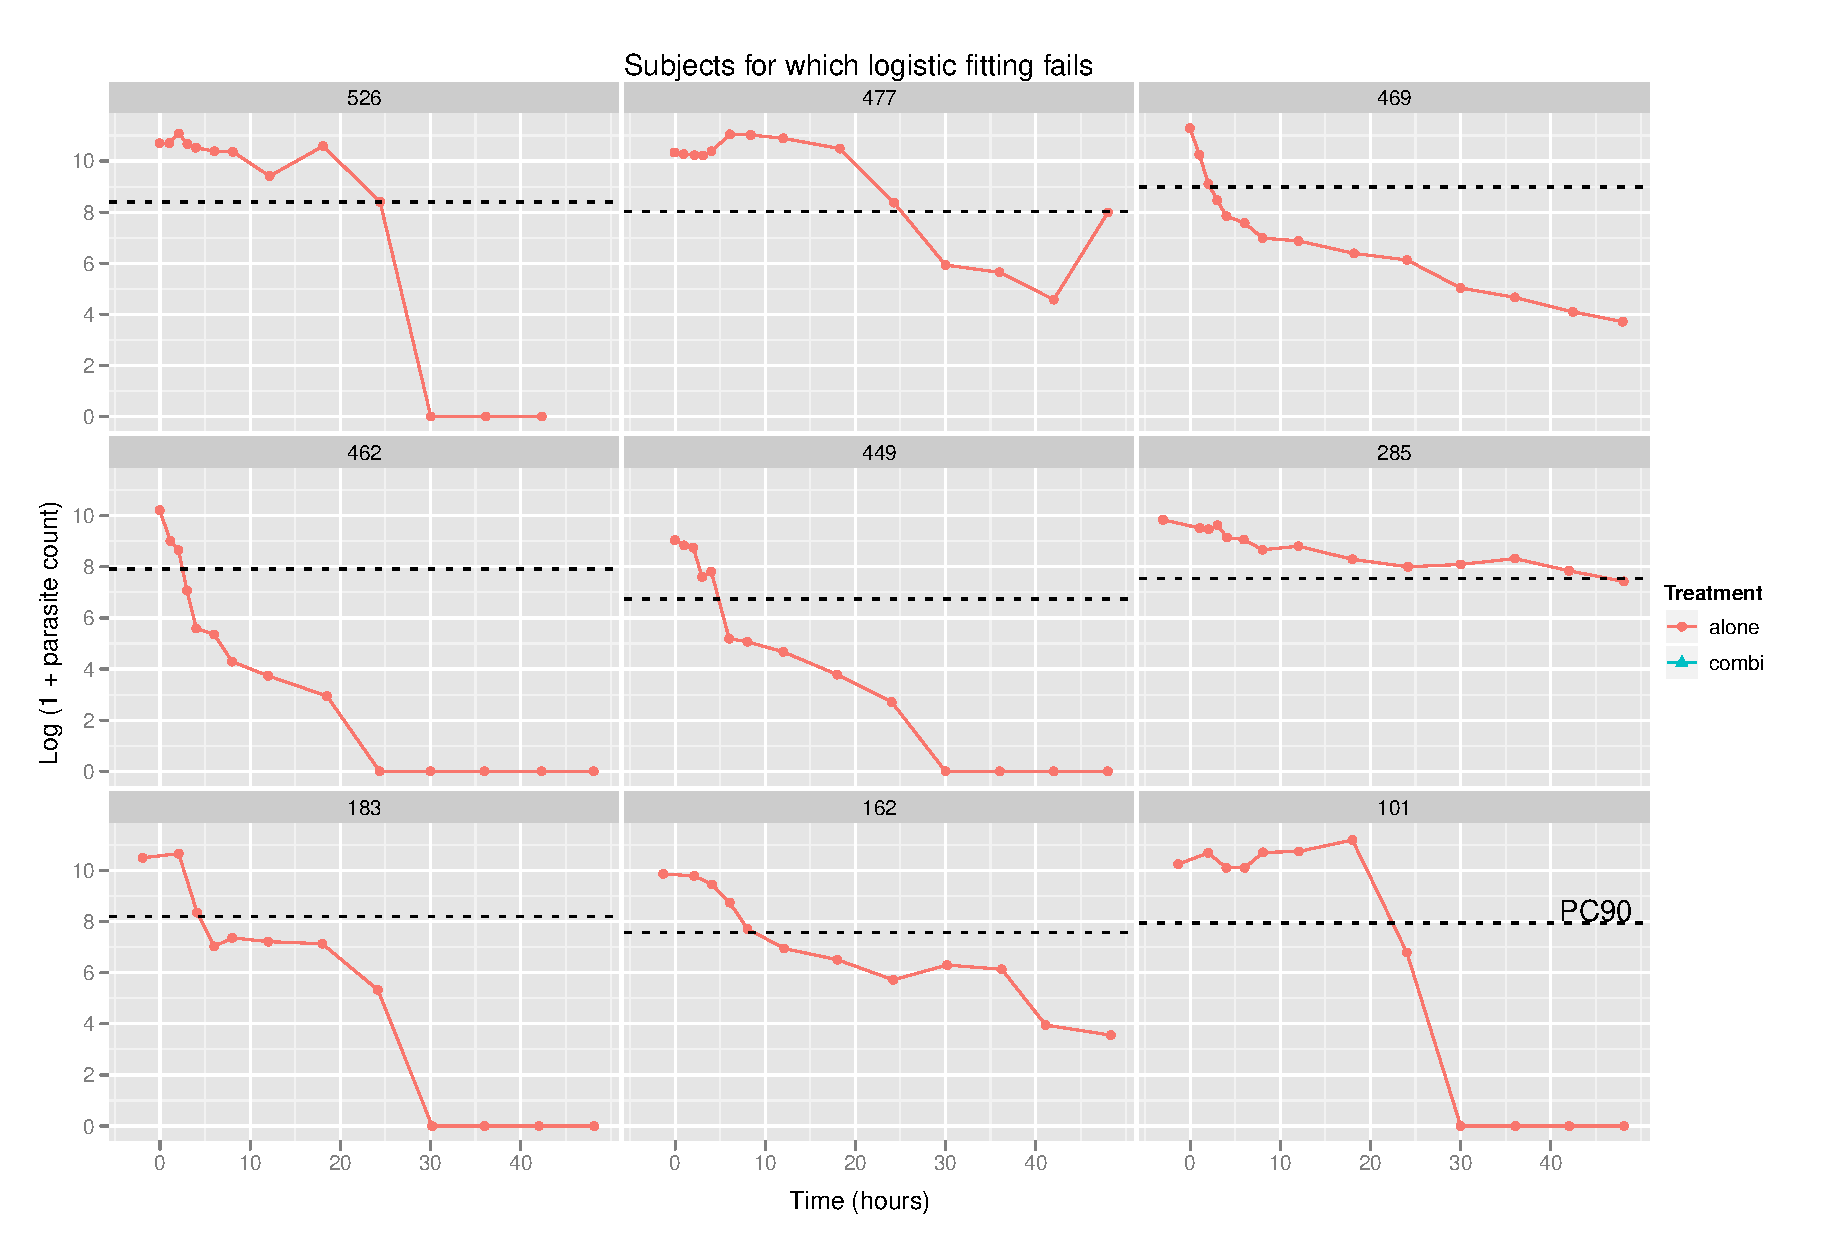
\includegraphics[width=6.1in]{failures.eps} 
\caption{Subjects for which the logistic fitting fails}\label{failures}
\end{figure}

In addition to parasite count profiles that simply do not conform to a logistic shape there were subjects where insufficient data in the region between the upper and lower asymptotes meant that logistic fitting was inappropriate. For example subjects 526 and 101 in Figure \ref{failures} where choice of different starting parameters for $\mu$ and $\beta$ would result in different logistic fits being obtained. One possible fit having a steep transition (large absolute $\beta$) whereby the data at the upper and lower levels is closely modeled. Another possible fit having a shallower transition (smaller $\beta$) that models the slope of a line passing through the ends of the run of points at the upper and lower levels and the point in the middle, but that has a less severe curvature such that the corners at the upper and lower levels are less well modeled. In summary the fit is free to rotate about the single point between the upper and lower levels and thus cannot be suitably defined.
\subsection{Log-linear interpolation}
The datum immediately above the PC90 level is joined with a straight line to the datum immediately below the PC90 level in on a plot of $\log(1+P_{t})$ against time. The point where this line crosses the PC90 level determines $t$=PC90.
\section{Comparison of estimation methods}
\subsection{Graphical comparison}
Figure \ref{pc90-agree} shows 8 examples of subjects where estimation by the 3 different methods shows good agreement. It seems likely that the differences between these estimates are comparable to experimental error. It can be seen that the 3 methods give close agreement when the data can be closely modeled by cubic or logistic fitting and when the gradient of the log-linear interpolation is similar to the regression models in the region around PC90. 
\begin{figure}[h]
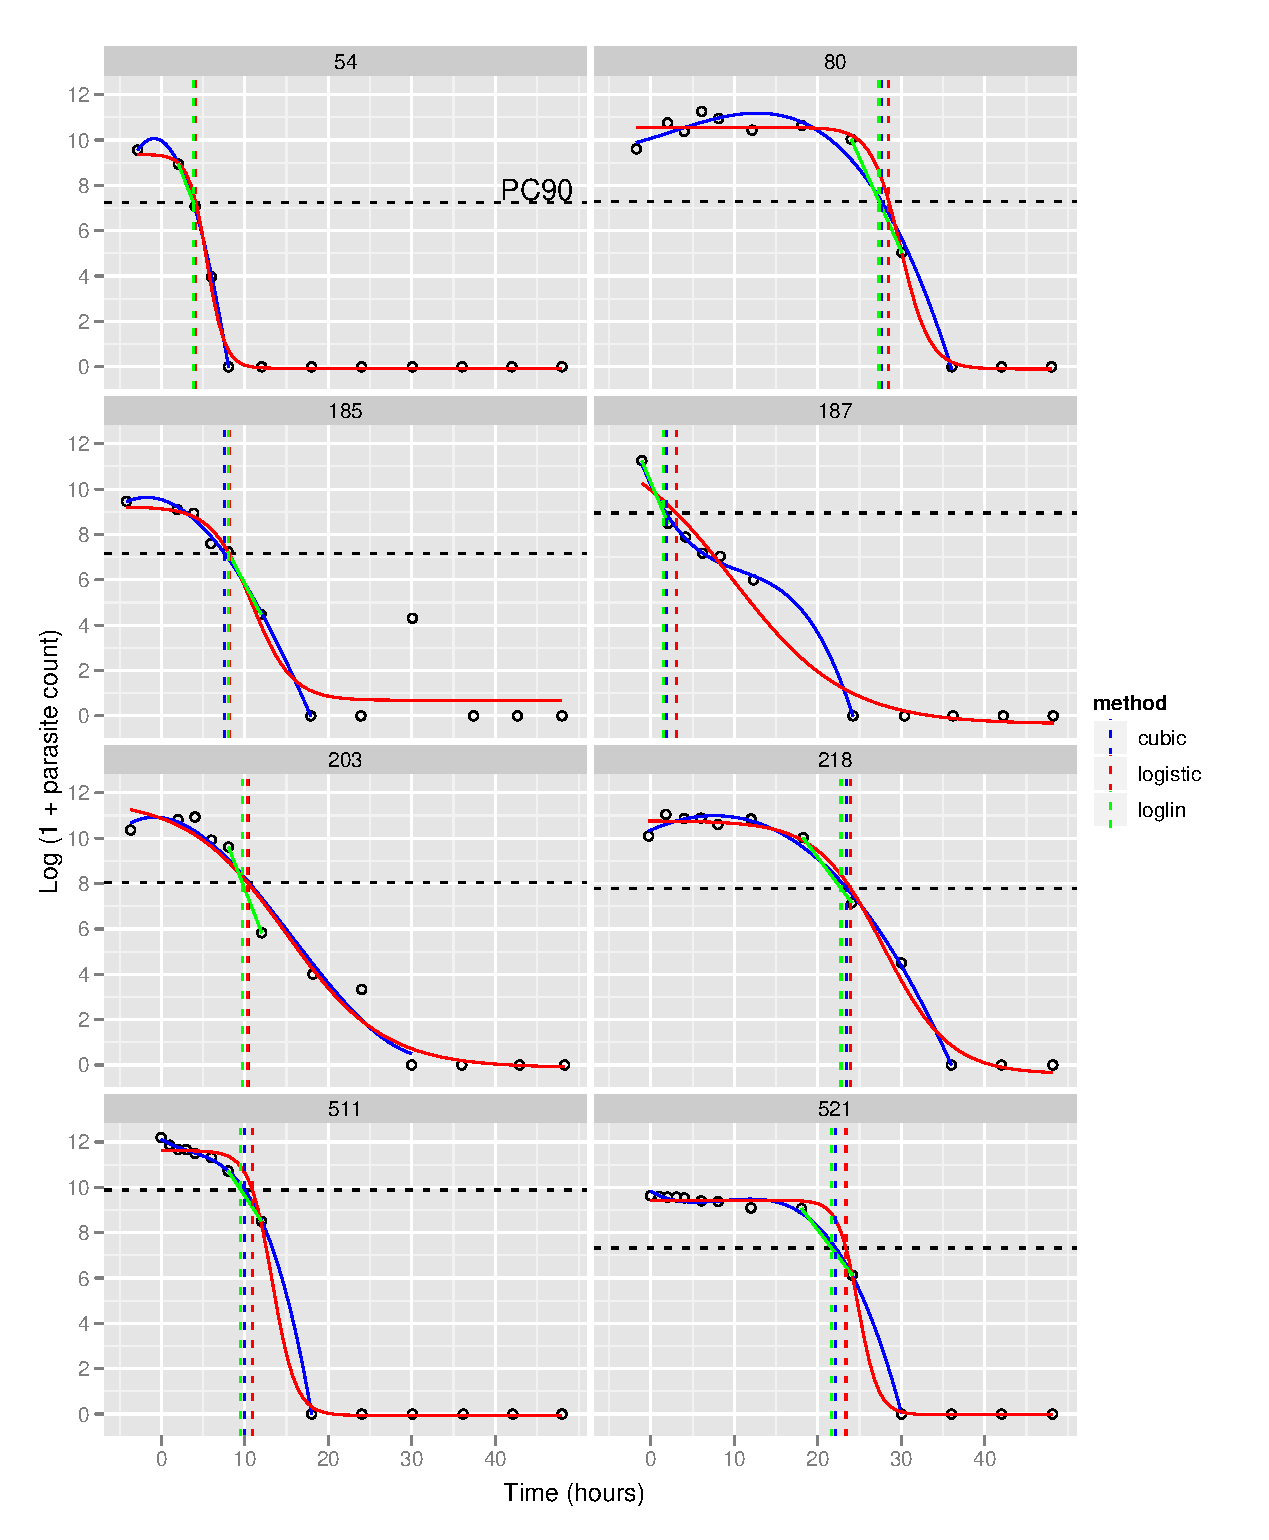
\includegraphics[width=6.5in]{pc90-agree.eps} 
\caption{Subjects with little difference in PC90 estimated by 3 methods}
\label{pc90-agree}
\end{figure}

Figure \ref{pc90-bad} shows examples of subjects where estimation by the 3 different methods has resulted in notable differences between PC90 estimates. These differences appear to arise when:
\begin{enumerate}
\item The drop in parasite count is slow or stationary around the PC90 level e.g. subjects 98, 453 and 509. In these cases the regression lines and interpolation may cross the PC90 level at markedly different times. In subject 509 this has given a difference in PC90 between the interpolation and cubic methods of almost 10 hours.
\item There is an ``unusual'' data near the PC90 level e.g. subjects 490 and 500 where recorded counts seemingly off the prevailing trend have influence the interpolated estimate.  
\end{enumerate}
\begin{figure}[h]
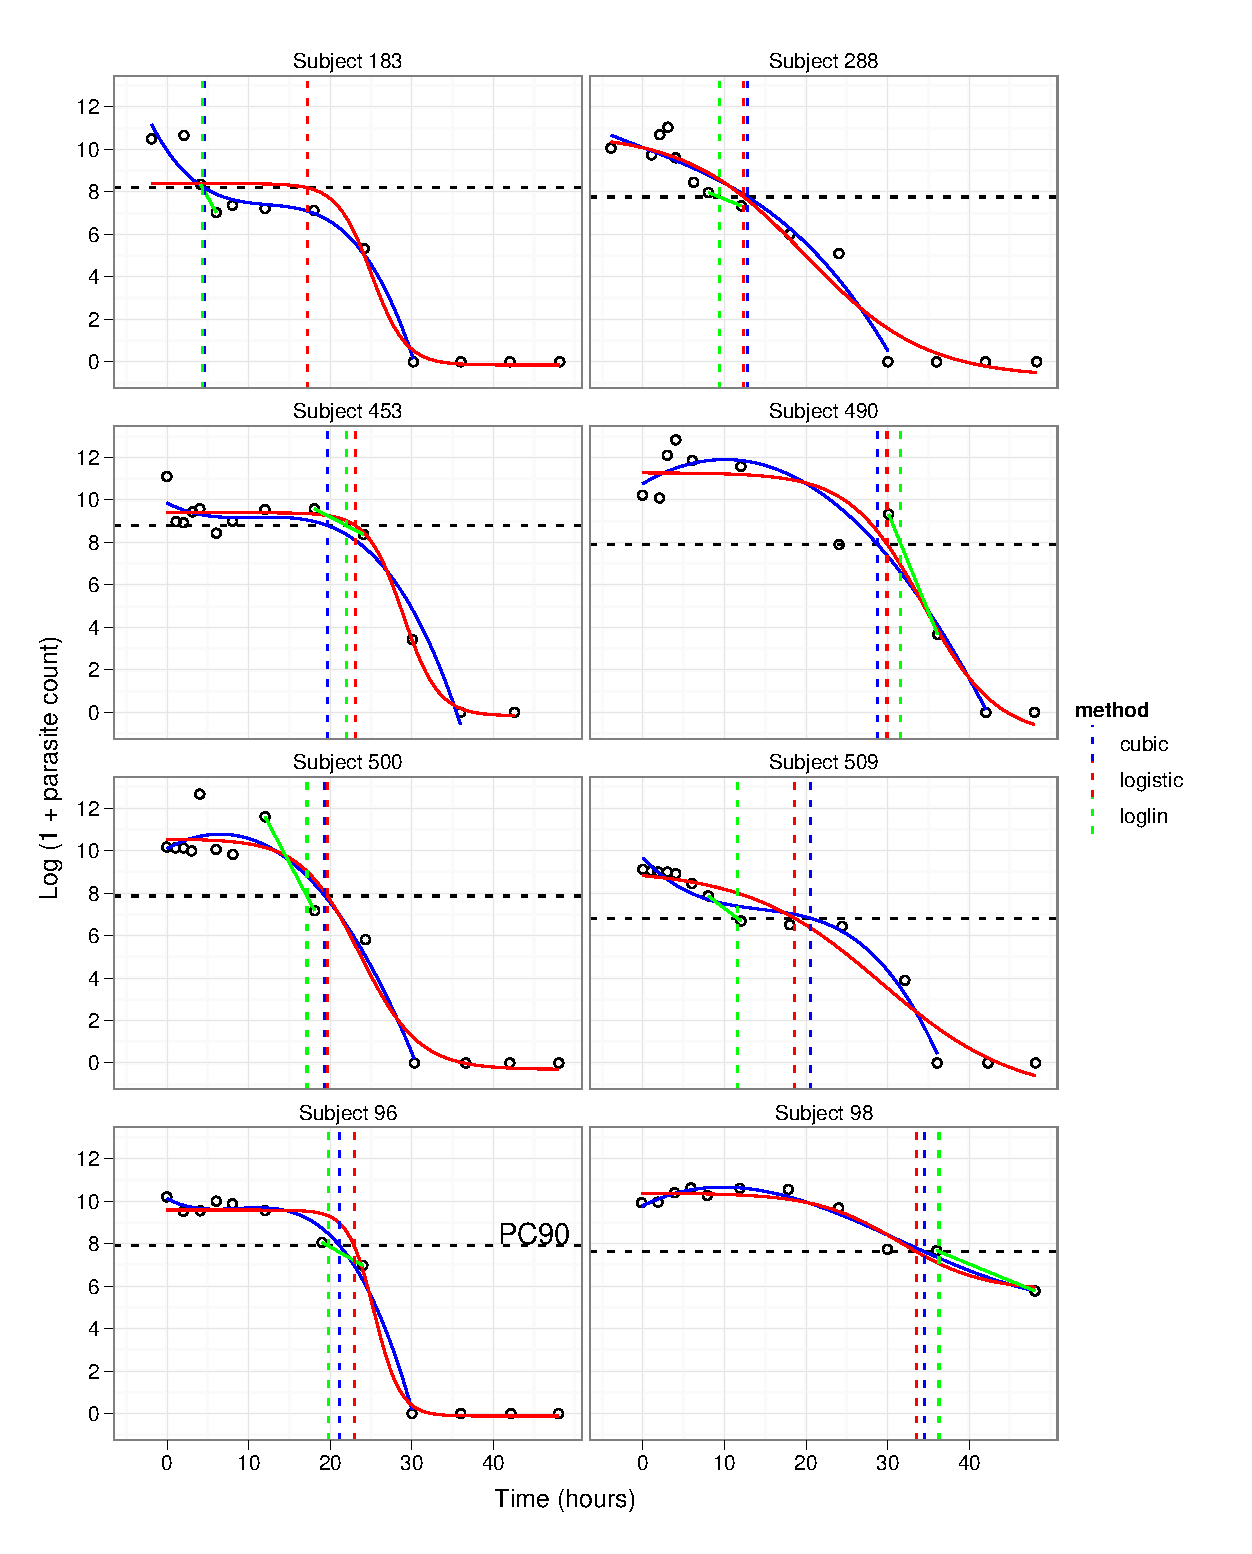
\includegraphics[width=6.5in]{pc90-bad.eps} 
\caption{Subjects with notable difference in PC90 estimated by 3 methods}
\label{pc90-bad}
\end{figure}
\begin{figure}[h]
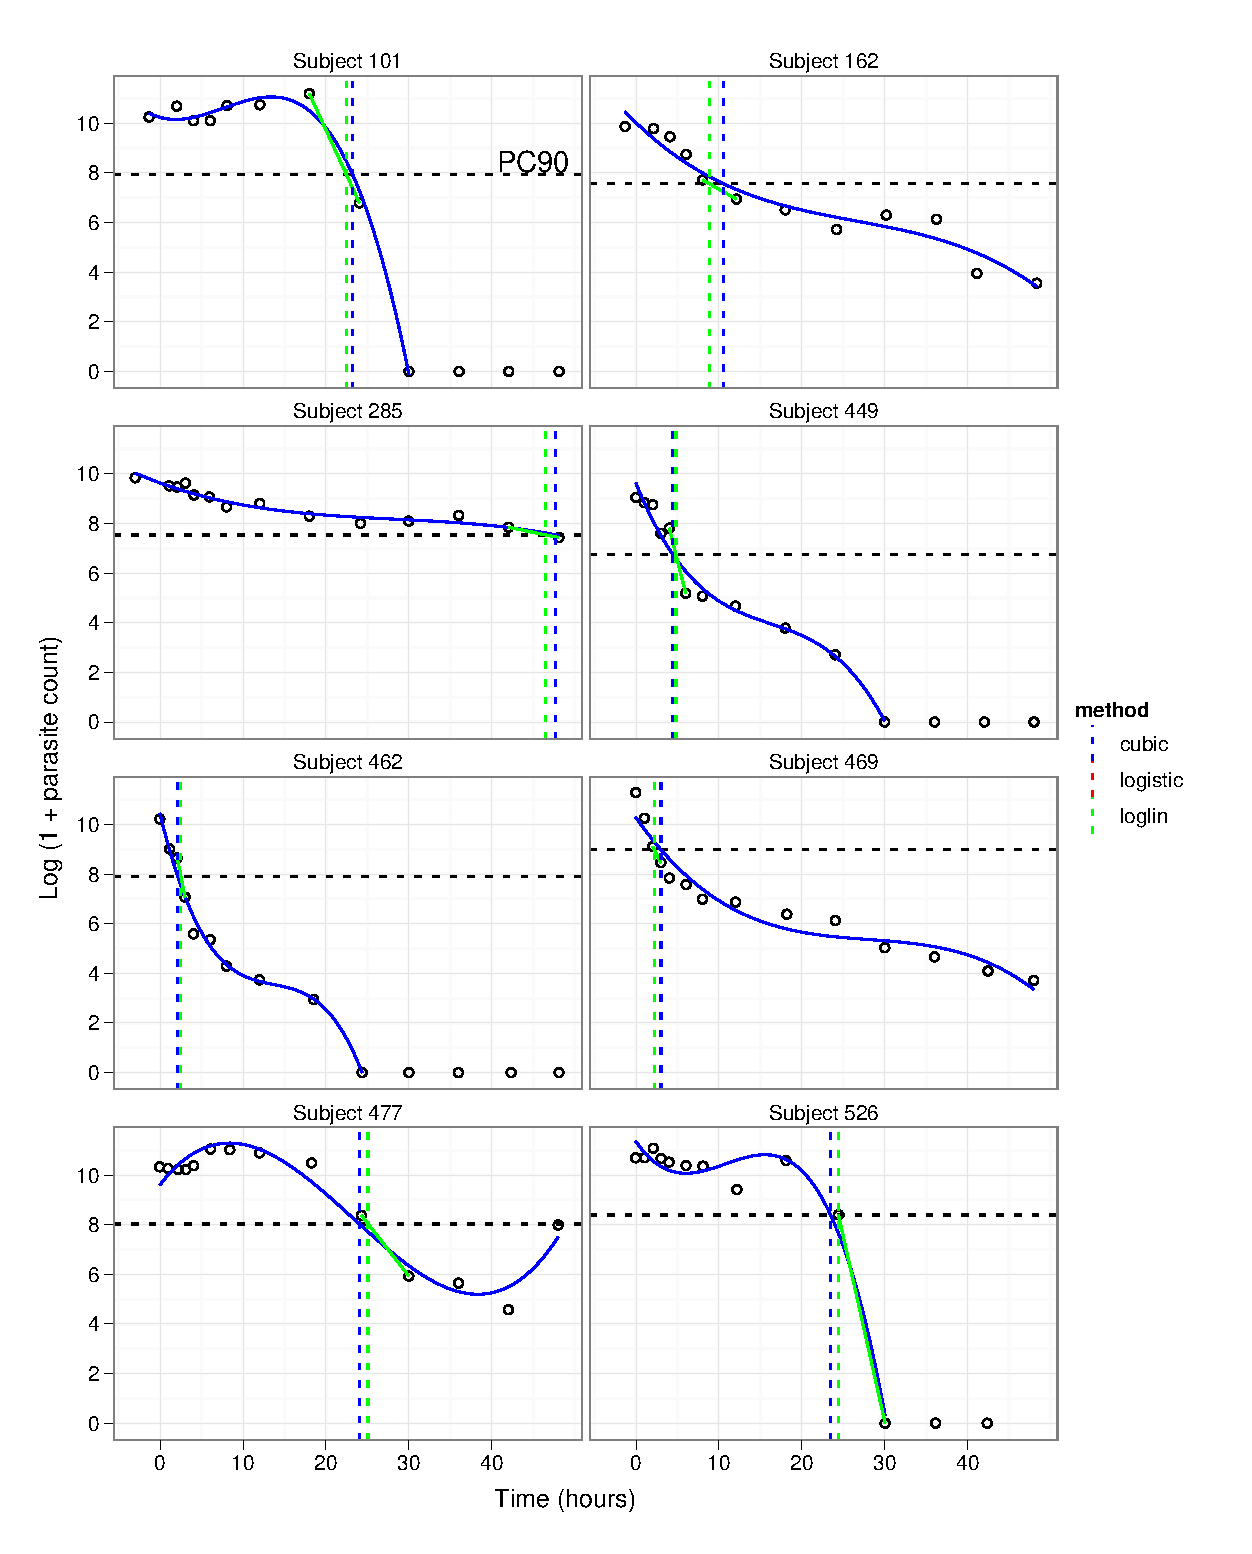
\includegraphics[width=6.5in]{pc90-nofit.eps} 
\caption{PC90 estimation for subjects where logistic fitting was inappropriate}
\label{pc90-bad}
\end{figure}
\clearpage
\subsection{Statistical comparison}
Table \ref{PC90} shows a comparison of the PC90 estimates by the 3 different methods utilised so far.
\begin{table}
\centering
\caption{Comparison of PC90 estimated by 3 methods}\label{PC90}
\begin{tabular}{|cccc|rrr|}
\hline
Subject&Centre&&&PC90&PC90&PC90\\
ID&ID&Sex&Treatment&cubic&logistic&log-linear\\
\hline
54&Centre 1&Male&alone&3.82&4.14&3.85\\
80&Centre 1&Male&alone&27.62&28.50&27.32\\
96&Centre 1&Female&alone&21.18&22.95&19.76\\
98&Centre 1&Male&alone&34.50&33.51&36.30\\
101&Centre 1&Female&alone&23.20&-&22.45\\
140&Centre 1&Male&combi&9.47&10.16&9.47\\
150&Centre 1&Female&alone&22.52&23.12&21.75\\
162&Centre 1&Male&alone&10.54&-&8.84\\
176&Centre 1&Male&combi&5.32&5.66&5.05\\
182&Centre 1&Female&combi&3.98&4.29&3.65\\
183&Centre 1&Male&alone&4.55&17.21&4.35\\
185&Centre 1&Male&combi&7.59&8.13&8.10\\
187&Centre 1&Male&alone&1.81&3.05&1.53\\
197&Centre 1&Female&combi&8.38&8.35&8.40\\
203&Centre 1&Female&combi&10.48&10.30&9.69\\
218&Centre 1&Male&combi&23.48&23.92&22.77\\
224&Centre 1&Male&alone&28.86&30.26&30.01\\
262&Centre 1&Male&combi&9.40&9.85&9.40\\
264&Centre 1&Female&combi&0.37&1.43&0.85\\
280&Centre 1&Female&combi&8.76&9.72&9.04\\
285&Centre 1&Female&alone&47.74&-&46.52\\
288&Centre 1&Female&combi&12.86&12.38&9.38\\
294&Centre 1&Male&combi&8.86&8.68&7.73\\
295&Centre 1&Male&alone&5.02&4.98&4.83\\
449&Centre 2&Male&alone&4.45&-&4.82\\
453&Centre 2&Female&alone&19.66&23.08&21.97\\
462&Centre 2&Female&alone&2.11&-&2.49\\
469&Centre 2&Male&alone&3.01&-&2.21\\
477&Centre 2&Female&alone&24.03&-&25.08\\
490&Centre 2&Female&alone&28.73&29.94&31.63\\
500&Centre 2&Male&combi&19.36&19.66&17.15\\
502&Centre 2&Female&combi&15.33&16.33&14.77\\
504&Centre 2&Female&alone&5.07&6.64&5.00\\
505&Centre 2&Female&combi&8.26&9.02&8.75\\
509&Centre 2&Male&alone&20.59&18.63&11.59\\
511&Centre 2&Male&combi&10.00&10.91&9.51\\
519&Centre 2&Male&combi&15.63&16.08&14.68\\
521&Centre 2&Female&alone&22.14&23.38&21.64\\
523&Centre 2&Female&combi&5.82&5.97&5.84\\
525&Centre 2&Female&combi&6.15&6.17&6.23\\
526&Centre 2&Female&alone&23.48&-&24.42\\
530&Centre 2&Male&alone&29.10&29.28&28.09\\
532&Centre 2&Male&combi&9.16&9.21&8.08\\
\hline
\end{tabular}
\end{table}
If we perform 2-way ANOVA between the 3 PC90 estimates by subject and method i.e.
$$\mathrm{PC}90_{ij}=subject_{i}+method_{j}+\epsilon_{ij}\quad\quad\epsilon\sim N(0,\sigma^{2})$$ 
we obtain the residuals shown in Figure \ref{pc90resid}.
\begin{figure}[h]
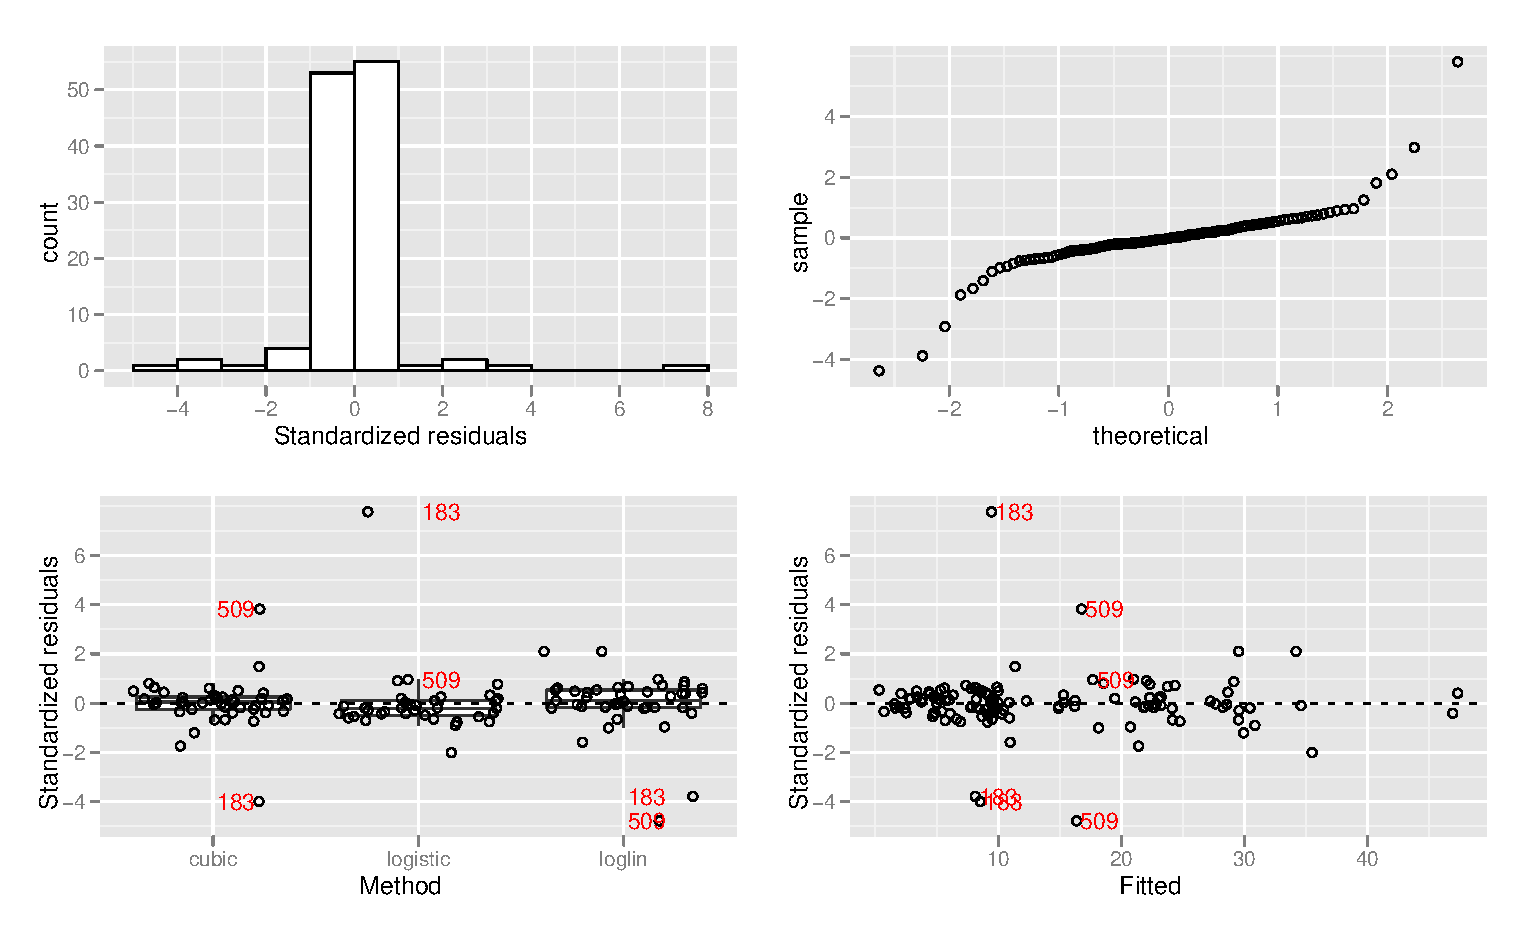
\includegraphics[width=6.5in]{pc90resid.eps} 
\caption{Residuals from ANOVA analysis of PC90 estimates}
\label{pc90resid}
\end{figure}
 It can be seen that there are several outlying data points at up to $5\sigma$. These correspond to subject  509 for whom we obtained very different PC90 estimates by the 3 methods. As can be seen in Figure \ref{pc90-bad}, this is due to the parasite count being fairly constant around the PC90 level for these subjects.

If we repeat the ANOVA analysis with subject 509 removed, we obtain the residuals shown in Figure \ref{pc90resid-sub}.
\begin{figure}[h]
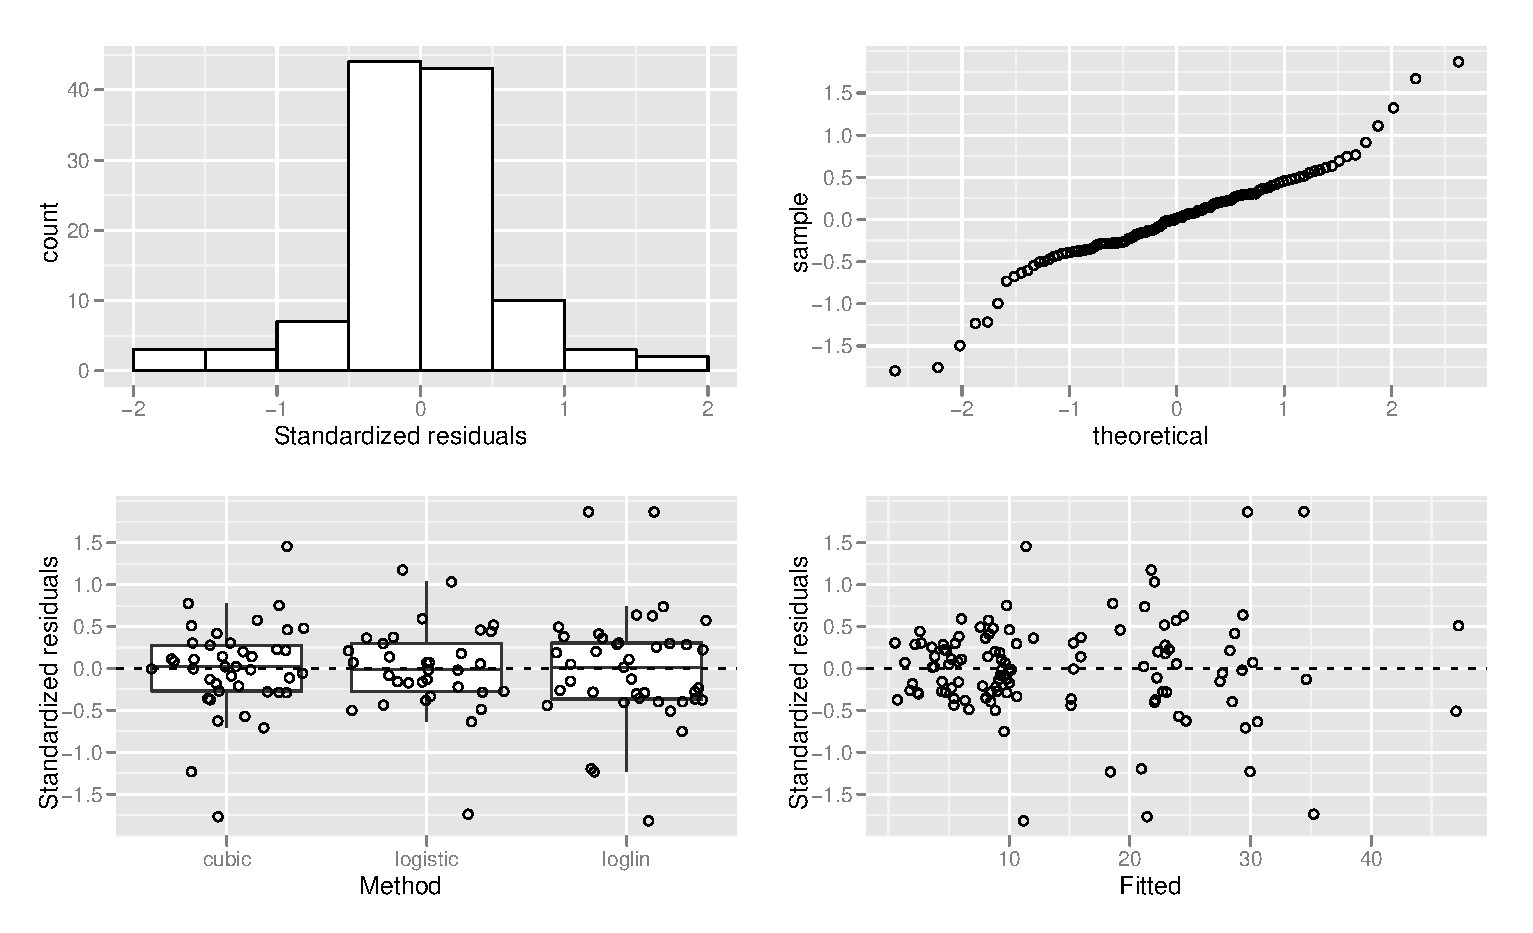
\includegraphics[width=6.5in]{pc90resid-sub.eps} 
\caption{Residuals from ANOVA analysis with subject 509 removed}
\label{pc90resid-sub}
\end{figure}
It can be seen that the residuals are approximately normally distributed with no obvious structure except for pehaps a smaller variance at smaller PC90 times. The results of the ANOVA analysis are shown in Table \ref{pc90aov}. There is evidence to reject the hypothesis that the 3 methods give the same PC90 values ($P<0.0005$). If we follow this up with 3 separate paired $t$ tests we find no evidence 
\begin{table}
\centering
\caption{ANOVA comparison of PC90 estimated by 3 methods}\label{pc90aov}
\begin{tabular}{l|rrrrr}
&D.O.F.&Sum Sq.&Mean Sq.&$F$&P($>F$)\\
\hline
subject&41&13896.8&338.9&574.85&$<2.2\times 10^{-16}$\\
method&2&11.3&5.6&9.58&0.00018\\
residual&82&48.3&0.6&&\\
\end{tabular}
\end{table}